\documentclass[11pt]{article}

\usepackage[margin=1in]{geometry}
\usepackage[T1]{fontenc}
\usepackage{lmodern}
\usepackage{microtype}
\usepackage{amsmath,amssymb,amsthm}
\usepackage{booktabs}
\usepackage{array}
\usepackage{tabularx}
\usepackage{float}
\usepackage{tikz}
\usepackage[hidelinks]{hyperref}

\usetikzlibrary{arrows.meta}

\newtheorem{theorem}{Theorem}
\newtheorem{observation}{Observation}
\newcommand{\delivers}{\mathrel{\to}}
\newcommand{\inflight}[2]{[#1\delivers #2]}

\title{\textbf{A Five-Node Periodic Execution in\\
Fixed-Delay Amnesiac Flooding}\\[0.35em]
\large A verification note concerning Open Problem 2 of Hussak and Trehan}
\author{Oscar Hong}
\date{23 July 2026}

\begin{document}

\maketitle

\begin{abstract}
Hussak and Trehan ask whether multi-source amnesiac flooding must terminate
on a bipartite graph when exactly one edge has a fixed transit time greater
than one round.  This note gives a candidate negative answer.  The graph is a
four-cycle with one pendant vertex, the two sources are nonadjacent, and one
cycle edge has transit time two.  A complete ten-round state certificate
shows that the nonempty state in round~5 recurs in round~10, so the execution
has period five and never terminates.  The certificate includes messages in
transit and uses the timing convention of the original paper.  A separate
four-cycle execution also appears to contradict Theorem~4.3 of that paper and
points to a specific failed transitivity step in its proof.  The purpose of
this note is to make both claims easy to check.
\end{abstract}

\section{Purpose and main claim}

In \emph{Termination of amnesiac flooding}, Hussak and Trehan pose the
following question \cite[Open Problem~2]{HT2023}:
\begin{quote}
Does amnesiac flooding from multiple sources on a bipartite graph, where
there is a fixed time of message transit greater than one round along a
single edge, terminate?
\end{quote}
The example below answers this question negatively, provided the round and
in-transit-state conventions in Section~\ref{sec:model} agree with those
intended in \cite{HT2023}.

\begin{theorem}\label{thm:main}
There is a finite connected bipartite graph with two simultaneous sources
and exactly one edge of fixed transit time two on which amnesiac flooding is
periodic and does not terminate.
\end{theorem}

The proof is a finite certificate.  No asymptotic argument or unreported
computer search is needed to check it.

\section{Model and state convention}\label{sec:model}

Let \(G=(V,E)\) be a finite undirected graph, and let \(I\subseteq V\) be the
set of sources.  The execution is synchronous.
\begin{enumerate}
  \item In round~1, every source sends the message to every neighbor.
  \item A message launched in round \(r\) on an edge of transit time \(w\)
        is delivered in round \(r+w-1\).  Thus, a unit-time launch is
        delivered in its launch round.
  \item For \(r\geq 1\), let
        \[
        R_r(v)=\{u:(u\delivers v)\text{ is delivered in round }r\}.
        \]
        If \(R_r(v)\neq\varnothing\), then in round \(r+1\), vertex \(v\)
        sends to every neighbor outside \(R_r(v)\), and to no neighbor in
        \(R_r(v)\).
  \item Messages moving in opposite directions on a delayed edge pass one
        another in transit.  They are not suppressed at an internal tick;
        suppression occurs only through the forwarding rule after delivery
        at an original vertex.
\end{enumerate}
These are the amnesiac forwarding rule and fixed-delay interpretation used
in Definition~1, Definition~5, and Figures~4--9 of \cite{HT2023}.

For each round \(r\), let \(D_r\) be the set of directed deliveries at
original vertices in that round.  Let \(F_r\) contain every message that,
after the launches and deliveries of round \(r\), is still in transit,
together with its direction and remaining transit time.  The \emph{full
state} is
\[
S_r=(D_r,F_r).
\]
The forwarding and transit rules determine \(S_{r+1}\) uniquely from
\(S_r\).  In the example below, the only delayed edge has transit time two,
so every message in \(F_r\) has exactly one round remaining.  We write
\(\inflight{x}{y}\) for such a message moving from \(x\) to \(y\).

\section{The five-node certificate}\label{sec:certificate}

Take
\[
V=\{a,b,c,d,e\},\qquad
E=\{ab,bc,cd,da,ae\}.
\]
Thus, \(a,b,c,d\) form a four-cycle and \(e\) is a leaf adjacent to \(a\).
The bipartition is
\[
\{a,c\}\ \big|\ \{b,d,e\}.
\]
Let the simultaneous source set be \(I=\{c,e\}\).  Assign transit time two
to \(ab\), in both directions, and transit time one to every other edge.

\begin{figure}[ht]
\centering
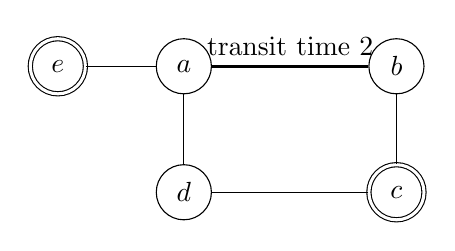
\begin{tikzpicture}[
  vertex/.style={circle,draw,minimum size=7mm,inner sep=0pt},
  source/.style={vertex,double,double distance=1.1pt},
  delayed/.style={line width=1.2pt},
  >=Latex
]
  \node[vertex] (a) at (0,1.6) {\(a\)};
  \node[vertex] (b) at (2.7,1.6) {\(b\)};
  \node[source] (c) at (2.7,0) {\(c\)};
  \node[vertex] (d) at (0,0) {\(d\)};
  \node[source] (e) at (-1.6,1.6) {\(e\)};

  \draw[delayed] (a) -- node[above] {transit time \(2\)} (b);
  \draw (b) -- (c);
  \draw (c) -- (d);
  \draw (d) -- (a);
  \draw (e) -- (a);
\end{tikzpicture}
\caption{The counterexample.  Double circles mark the two sources.  Every
unlabelled edge has transit time one.}
\label{fig:counterexample}
\end{figure}

\subsection*{Complete state table}

The execution is listed in Table~\ref{tab:main-states}.  An empty in-transit
column means \(F_r=\varnothing\).

\begin{table}[H]
\centering
\small
\renewcommand{\arraystretch}{1.18}
\begin{tabularx}{\textwidth}{
  @{}>{\raggedleft\arraybackslash}p{0.07\textwidth}
  >{\raggedright\arraybackslash}X
  >{\raggedright\arraybackslash}p{0.28\textwidth}@{}}
\toprule
Round \(r\) & Deliveries \(D_r\) & In transit \(F_r\)\\
\midrule
1  & \(\{c\delivers b,\ c\delivers d,\ e\delivers a\}\)
   & \(\varnothing\)\\
2  & \(\{a\delivers d,\ d\delivers a\}\)
   & \(\{\inflight{a}{b},\ \inflight{b}{a}\}\)\\
3  & \(\{a\delivers b,\ a\delivers e,\ b\delivers a,\ d\delivers c\}\)
   & \(\{\inflight{a}{b}\}\)\\
4  & \(\{a\delivers b,\ a\delivers d,\ a\delivers e,\ b\delivers c,\
       c\delivers b\}\)
   & \(\varnothing\)\\
5  & \(\{c\delivers d,\ d\delivers c\}\)
   & \(\varnothing\)\\
6  & \(\{c\delivers b,\ d\delivers a\}\)
   & \(\varnothing\)\\
7  & \(\{a\delivers e\}\)
   & \(\{\inflight{a}{b},\ \inflight{b}{a}\}\)\\
8  & \(\{a\delivers b,\ b\delivers a\}\)
   & \(\varnothing\)\\
9  & \(\{a\delivers d,\ a\delivers e,\ b\delivers c\}\)
   & \(\varnothing\)\\
10 & \(\{c\delivers d,\ d\delivers c\}\)
   & \(\varnothing\)\\
\bottomrule
\end{tabularx}
\caption{The full flooding state for rounds 1 through 10.  In
\(\inflight{x}{y}\), the message has one round of transit remaining.}
\label{tab:main-states}
\end{table}

\begin{proof}[Proof of Theorem~\ref{thm:main}]
The graph in Figure~\ref{fig:counterexample} is finite, connected, and
bipartite under the displayed bipartition.  It has two nonadjacent sources
and exactly one delayed edge.

We first check the only less immediate transitions.  In round~1, source \(c\)
sends to \(b,d\), and source \(e\) sends to \(a\), giving the first row of
Table~\ref{tab:main-states}.  In round~2, \(a\) excludes \(e\) and sends to
\(b,d\); \(b\) excludes \(c\) and sends to \(a\); and \(d\) excludes \(c\)
and sends to \(a\).  The two launches on \(ab\) remain in transit, while the
two launches on unit-time edge \(ad\) are delivered immediately.  This gives
the second row.

In round~3, the two messages already travelling on \(ab\) are delivered.
The round-2 delivery \(d\delivers a\) also causes \(a\) to launch a new
message toward \(b\), which remains in transit, and to deliver one to \(e\).
Likewise, \(a\delivers d\) causes \(d\delivers c\).  This gives the third
row.  In round~4, the remaining delayed message is delivered at \(b\);
applying the same exclusion rule to the round-3 receiver sets gives the
other four deliveries shown.  Every later row follows directly by the same
rule.

The last row is identical to the fifth row:
\[
S_5=\bigl(\{c\delivers d,d\delivers c\},\varnothing\bigr)=S_{10}.
\]
Because the full-state transition is deterministic,
\(S_{5+k}=S_{10+k}\) for every \(k\geq 0\).  Each state in rounds \(5\)
through \(9\) is nonempty.  That five-round block therefore repeats forever,
so flooding never terminates.
\end{proof}

\section{A separate weighted-cycle check}\label{sec:cycle}

The main counterexample does not rely on Theorem~4.3 of \cite{HT2023}.
There is, however, a smaller periodic execution on an edge-weighted cycle.
This provides an independent diagnostic for the model interpretation and
reveals an apparent gap in the proof of that theorem.

Take the four-cycle in cyclic order
\[
0,\ 2,\ 1,\ 3,\ 0,
\]
with source set \(I=\{0,1,2\}\).  Give edge \(02\) transit time two and every
other edge transit time one.  Table~\ref{tab:cycle-states} uses the same
state convention as Table~\ref{tab:main-states}.

\begin{table}[H]
\centering
\small
\renewcommand{\arraystretch}{1.16}
\begin{tabularx}{\textwidth}{
  @{}>{\raggedleft\arraybackslash}p{0.07\textwidth}
  >{\raggedright\arraybackslash}X
  >{\raggedright\arraybackslash}p{0.28\textwidth}@{}}
\toprule
Round \(r\) & Deliveries \(D_r\) & In transit \(F_r\)\\
\midrule
1 & \(\{0\delivers3,\ 1\delivers2,\ 1\delivers3,\ 2\delivers1\}\)
  & \(\{\inflight{0}{2},\ \inflight{2}{0}\}\)\\
2 & \(\{0\delivers2,\ 1\delivers3,\ 2\delivers0\}\)
  & \(\{\inflight{2}{0}\}\)\\
3 & \(\{0\delivers3,\ 2\delivers0,\ 2\delivers1,\ 3\delivers0\}\)
  & \(\varnothing\)\\
4 & \(\{1\delivers3,\ 3\delivers1\}\)
  & \(\varnothing\)\\
5 & \(\{1\delivers2,\ 3\delivers0\}\)
  & \(\varnothing\)\\
6 & \(\varnothing\)
  & \(\{\inflight{0}{2},\ \inflight{2}{0}\}\)\\
7 & \(\{0\delivers2,\ 2\delivers0\}\)
  & \(\varnothing\)\\
8 & \(\{0\delivers3,\ 2\delivers1\}\)
  & \(\varnothing\)\\
9 & \(\{1\delivers3,\ 3\delivers1\}\)
  & \(\varnothing\)\\
\bottomrule
\end{tabularx}
\caption{A period-five execution on a weighted four-cycle.  Note that
round~6 is not a terminating state because two messages remain in transit.}
\label{tab:cycle-states}
\end{table}

Here \(S_4=S_9\neq(\varnothing,\varnothing)\), so the cycle execution is
periodic with period five.  This appears to contradict the termination claim
in \cite[Theorem~4.3]{HT2023}.

\subsection*{The transitivity step}

The proof of Theorem~4.3 expands a weighted cycle by inserting tick vertices.
It labels the expanded cycle modulo its total weight \(\sigma\), and defines
a relation on source vertices by
\begin{equation}\label{eq:relation}
v\sim w
\quad\Longleftrightarrow\quad
\exists m\;[\,v+m=w-m\ \text{ and }\ v+m\in G\,],
\end{equation}
where \(G\) denotes the original vertices, not the inserted ticks.  The proof
claims that this relation is transitive.  From witnesses \(m'\) for
\(v\sim w\) and \(m''\) for \(w\sim z\), it obtains
\[
v+(m'+m'')=z-(m'+m'').
\]
The equality is valid, but it does not establish the second condition in
\eqref{eq:relation}: the new meeting point need not be an original vertex.

The cycle above gives a direct failure.  Its expanded cyclic order is
\[
(0,t,2,1,3),
\]
where \(t\) is the sole tick.  Assign these vertices positions
\(0,1,2,3,4\) modulo \(5\).  The original-vertex positions are
\(\{0,2,3,4\}\), and the source positions are \(\{0,2,3\}\).  In the
following calculation, source vertices are denoted by their positions rather
than their original labels.  Equation
\eqref{eq:relation} gives
\[
0\sim3 \quad(m'=4,\ \text{meeting point }4),\qquad
3\sim2 \quad(m''=2,\ \text{meeting point }0).
\]
But \(0\not\sim2\): the unique solution of \(0+m=2-m\pmod 5\) is \(m=1\),
whose meeting point is the tick at position \(1\).  Hence \(\sim\) is not
transitive on this instance.  The equivalence-class counting argument that
starts with equation~(20) of \cite{HT2023} therefore does not apply as
written.

\clearpage
\section{Checks and questions for verification}

The two state tables were checked in three ways: by direct transition audit,
by a dependency-free deterministic simulator retaining every in-transit
message, and by an independent reimplementation of the transition rule.  As
a timing calibration, the simulator also reproduces the repeated flooding
state in rounds~5 and~13 reported for Figure~6 of \cite{HT2023}.  The tables
in this note remain complete, independently checkable certificates.

The points on which author verification would be most valuable are:
\begin{enumerate}
  \item Does Section~\ref{sec:model} match the intended round timing and
        tick behavior of \cite{HT2023}?
  \item Is every transition in Table~\ref{tab:main-states} valid under that
        model, making \(S_5=S_{10}\) a negative answer to Open Problem~2?
  \item Is the weighted-cycle execution in Table~\ref{tab:cycle-states}
        valid, and does the tick midpoint above invalidate the claimed
        transitivity in the proof of Theorem~4.3?
  \item Is either example already known, or covered by a correction or
        result not cited here?
\end{enumerate}

\paragraph{Computational assistance.}
AI-assisted finite-state search was used to locate small candidate examples.
The resulting claims are stated here as explicit state certificates, and the
proof of Theorem~\ref{thm:main} does not depend on the search procedure.

\begin{thebibliography}{1}

\bibitem{HT2023}
Walter Hussak and Amitabh Trehan.
\newblock Termination of amnesiac flooding.
\newblock \emph{Distributed Computing}, 36:193--207, 2023.
\newblock \url{https://doi.org/10.1007/s00446-023-00448-y}.

\end{thebibliography}

\end{document}
